\section{Evaluation Methodology}% Effectiveness of \approachName}
\label{sec:methodology}
We now describe a detailed methodology to experimentally judge how well a query optimizer chooses query plans. We describe this methodology as we use it to assess the effectiveness of MongoDB's \approachName query optimizer --- but note that this approach is not limited to \approachName query optimization, or even to document store optimisation, as it makes no assumptions about the internal workings of the query optimizer. We also describe the visual presentations we use to present the results. %Through this experiment, we find that the query optimizer does not consider collection scan as a candidate query plan; even when it does, it sticks on index scan while collection scan is actually a better choice.  In the next section, we focus on reveal the impact of this issue, and explore the underlying mechanism of \approachName to identify the root cause. 


\subsection{Testing Setup}
The testing environment adopts a typical client-server architecture. A single client communicates with a \relname server that is deployed on an Amazon EC2 (Elastic Compute Cloud) instance. The instance type we chose is \verb|m6i.large|. M6 instances work well with Amazon EBS (Amazon Elastic Block Store) gp3 (general purpose SSD) volumes for instance block storage. Gp3 is the default EBS volume type for Amazon EC2 instances and provides baseline performance of 3,000 IOPS per volume, regardless of volume size, to meet the performance needs of most applications. 100GB of storage is sufficient for storing our database and metadata. During experiments, we need to make sure that RAM is not the bottleneck. For the most stable and fastest processing, we need to ensure that our indexes fit entirely in RAM so that the system can avoid reading the index from disk. The instance type we use has 16GB RAM, which is more than enough to keep all indexes in memory for the workloads we used during testing.

\begin{comment}
\af{Where is the client deployed? what hardware, network characteristics to server?}
\end{comment}

We wrote a Python client application to run the experiments and visualize the results. The client runs on the same instance as the server because the client is idle while queries are running, and the network latency is not relevant for our tests. This evaluation client executes each query and gathers execution statistics from the database using MongoDB's query language. After the testing is complete, this client also analyzes statistical information and visualizes the results.

%\subsection{MongoDB Setup, Database Content, Queries}
\subsection{MongoDB Setup and Database Content}
The command line interface and the configuration file provide MongoDB administrators with many options and settings to control the operation of the database system.  We modify the default configuration file \verb|mongod.conf| to  allow  remote  access,  since our  Python  application  runs  on  the client side. During the experiment, we use the \verb|cursor.explain()| method with \verb|allPlansExecution| mode to inspect query plan candidates and execution statistics. 

The experiments we show here use one collection that contains $1 \times 10^5$ documents. Each document has two fields, namely A and B. A positive integer in the range $[0, 1\times 10^5)$ is assigned to each field. Different experiments use different choices for the distribution of the fields and for the index structures. For example, in the first experiment of Section~\ref{sec:evaluation}, fields A and B both have uniform distribution and the same cardinality with $10^5$ distinct values, no repetitions among the documents, and we create indexes A\textunderscore1 and B\textunderscore1 on fields A and B, respectively.

Despite the simplicity of this data model, the experimental setup exercises the core of MongoDB's query optimizer. As described in Section~\ref{sec:candidate-plan-generation}, MongoDB generates candidate query plans based on the access methods available for the documents required by the query. With a few exceptions, which are not relevant in these experiments, the optimiser does not consider reordering query stages or multiple join strategies. This keeps the set of candidate plans small, but means that queries must be constructed carefully to perform well\footnote{\url{https://www.red-gate.com/simple-talk/blogs/enjoying-joins-in-mongodb/}}. Further, while we focus on simple queries involving two fields so that the visualizations correspond directly to the data, this approach can be applied to any query where the optimal plan depends on the cardinality of two or more subqueries.

\subsection{Query Template}
In order to assess the effectiveness of the query optimizer, we use conjunctive range queries of the following form:
$$ \sigma [ \mathit{lowA} \le A < \mathit{highA} \wedge \mathit{lowB} \le B < \mathit{highB} ] ( \mathit{Collection} ) $$

These are selection queries with two range predicates that allow us to have detailed control over the query selectivity. All the queries we apply have the same shape, finding all documents whose A field lies within a given range, and also the B field value lies in another range. The ranges are set by parameters $\mathit{lowA}$, $\mathit{highA}$, $\mathit{lowB}$, $\mathit{highB}$ whose values determine the selectivities of a particular query of this shape. The queries are then executed using MongoDB's query language, as shown in \autoref{algo:queryshape}.

\begin{lstlisting}[caption=Query Shape in MongoDB Query Syntax, label=algo:queryshape]
db.collection.find({
    "A" : {"$gte" : lowA, "$lt" : highA},
    "B" : {"$gte" : lowB, "$lt" : highB}
})
\end{lstlisting}

We can determine the selectivity for range predicate on field $X$, $e_X$, 
using the following formula:
\begin{align}
\begin{split}
 e_X= \frac{\textit{numbers of documents satisfying range 
 predicate on field X}}{\textit{total number of documents}} \\
 \end{split}
\end{align}

\subsection{Methodology}
For each experiment, we create a single client and an Amazon EC2 instance with \relname installed. We then build a database with the appropriate data distribution and create the indexes for the particular experiment.

Then, the client performs queries that have different selectivity on A and B. More specifically, each query initiated by the client is a conjunction of one range predicate on A and the other on B.

For each query, the client records the selectivity for the range predicates on field A \& B, the execution plan, and the time taken to execute the plan. 

The client generates random queries of the given shape, picking random values for the parameters, to circumvent any potential workload prediction strategies by the query optimizer. For each query, the client determines and tracks the selectivity of the predicate on field A, and the selectivity of the predicate on field B. The query is then submitted to MongoDB, and the optimizer determines the query plan using \approachName and executes the chosen plan. We have disabled query plan caching for these experiments, so that MongoDB repeats optimization for every submitted query. The client determines which execution plan MongoDB chose for the query, using the MongoDB \verb|explain| method.

We also determine the runtime cost of each reasonable query plan, so that we can determine which is really the best (and thus we will see whether or not MongoDB is choosing wisely). %As we mentioned in Section~\ref{sec:hint}, 
MongoDB provides users with a \verb|hint(<queryPlan>)| method to customize execution plan selection. We use this method to force the query optimizer to execute each suitable plan. We run each plan ten times; when doing this, we extract the \texttt{execution\-Stats.\-execution\-Time\-Millis} field to retrieve
the wall-clock time in milliseconds required for each query execution. We then average the execution times for a plan and identify the optimal query plan: the one with the lowest average execution time among the possible plans for this query.

\paragraph{\textbf{Outlier handling.}} When we gathered execution times of all query plans, we noted
that there were a few outliers which deviate markedly from other data points. These outliers are
%usually fifty 
many times higher than the mean value. We assume that the likely cause is delays during MongoDB warm-up and unstable performance of our EC2 instances rather than the inherent faults of the benchmarked database. Therefore, we identify these outliers and drop them using the standard 1.5 IQR (interquartile range) rule: We measure the interquartile range  and drop any data point greater than the sum of the third quartile value and 1.5 times IQR, also we drop any measurement less than the first quartile minus 1.5 time IQR.

\paragraph{\textbf{Accuracy and Impact Metrics.}}
We finally assess the effectiveness of a query optimizer by two metrics: 
The measure of the overall success of MongoDB's optimizer is its \emph{accuracy}: the fraction of queries for which the optimizer's chosen plan is actually the best one.

In addition to finding whether or not MongoDB's \approachName optimizer chooses the best plan, we also want to know how much query performance is affected by the choice. If the chosen plan were only slightly slower than the best possible plan, users might find this quite acceptable, but if MongoDB chooses a plan that is much slower than another, this is more serious. So, for each query, we determine the ratio of the runtime of the plan chosen by the optimizer to the runtime of the plan which actually runs fastest for that query. We can consider this for each query, and we also calculate the average over all the queries we use, as the \emph{impact} of the optimizer.

%If there are multiple query plan candidates, we determine the real best candidate by measuring and comparing the execution time of each query plan candidate.  After executing all query plans,the one with the shortest execution time is the real best query plan.
%In this experiment, we aim to demonstrate that the query optimizer does not consider collection scan as a candidate query plan; even it does, it sticks on index scan while collection scan is theoretically a better choice. Therefore, we have two versions of MongoDB:

%\begin{description}
%     \item[V1] The original MongoDB with build version 
%     \mdbver.
%    \item[V2] We modify the source code of MongoDB \mdbver
%     so that the modified version considers the collection 
%     scan as a candidate plan. 
%\end{description}

% To begin with, we prove that V1 fails to perform collection scan as opposed to our expectation through visualizations. Furthermore, we repeat the experiment with V2 and yield newvisualization results. last but not least, we demonstratethat the current implementation has a preference bias through a comparison between results of V1 and V2. Finally,We conclude that \approachName has a preference bias since it sticks on index scans and underrates collection scans.

%The visualization reflect how an execution vary with respect to query selectivity. Recall that selectivity is a floating-point value (between zero and one) which represents the percentage of rows for which the query (and each filter in the query) is expected to return. We pick selectivity as one of the most crucial measurement since the majority of relational database systems consider selectivity as the mainfactor which determines the most efficient way to execute a given query \cite{lahdenmaki2005relational}, a.k.a. "access path" in RDBMS or "execution plan" in MongoDB. In Surajit Chaudhuri's work \cite{babcock2005towards}, he stated that  the robustness of RDBMS relies on quick and precise selectivity estimations. 

%The experiment is set up by installing \relname on an Amazon Elastic Compute Cloud (Amazon EC2) instance. A Python client will establish a connection to the instance.Then, the client performs queries which have different selectivity on A and B. More specifically, each query initiated by the client is a conjunction of one range predicate on A and the other one on B.

%For each query, the client records the selectivity for the range predicates on field A \& B, the execution plan, and the time consumption of seeking and executing the plan. 

%Then, the execution plan of each query is mapped to a position in a grid according to its selectivity on the field A and field B. In section \ref{sec:vm} we explainmore details about the mapping and visualization technique. When the experiment is done, the client willvisualize the result. The influence of query plan caches is eliminated by forcing MongoDB not to use them. 


\begin{figure}[thb]
  \centering
  %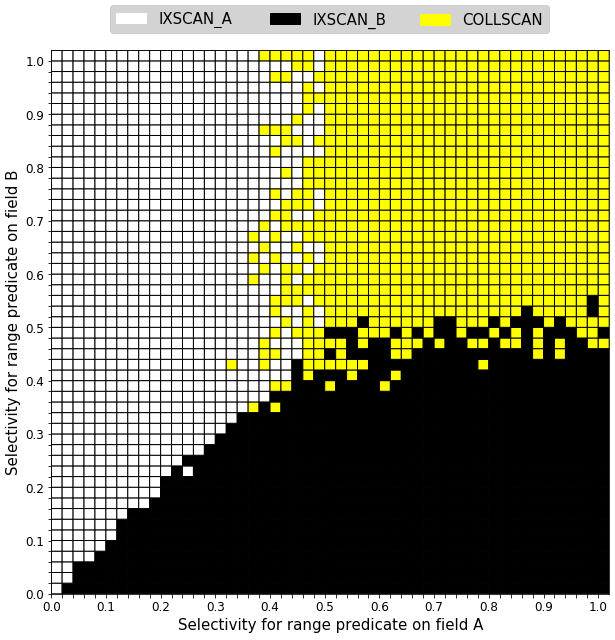
\includegraphics[width=0.7\linewidth]{images/body/gird_sample_1_toplegend.png}
  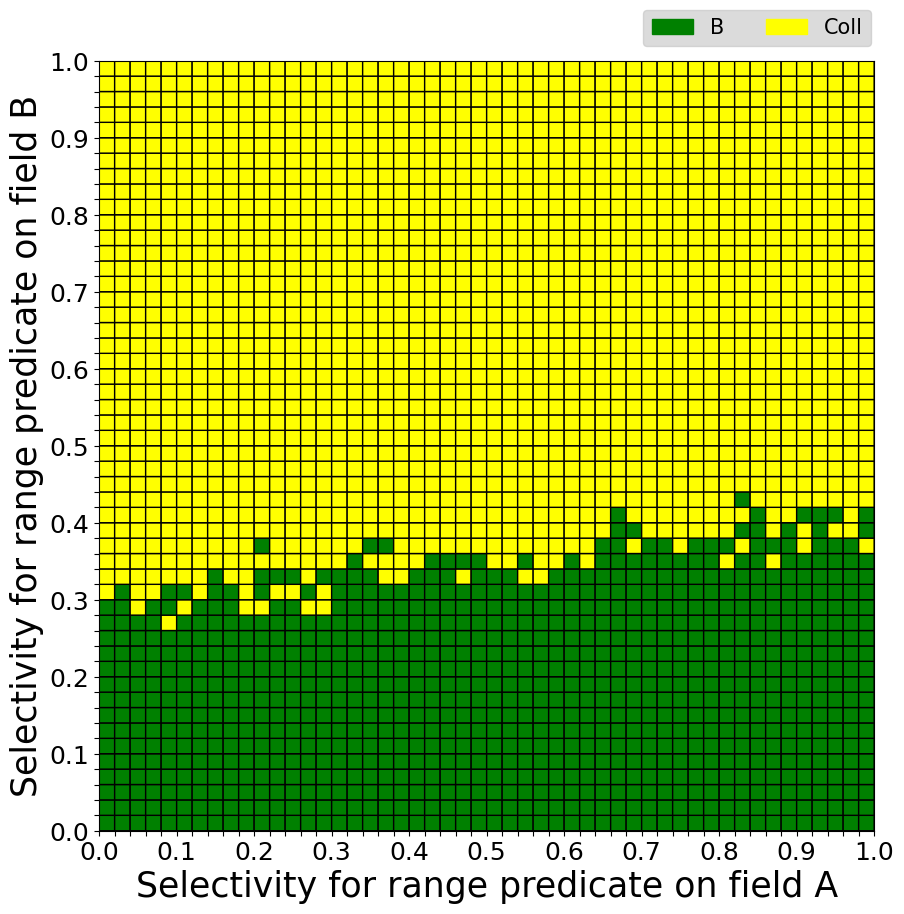
\includegraphics[width=0.7\linewidth]{images/results-without-covering-index/v\mdbver/comprehensive_practical_winner.png}
  \vspace*{-0.5\baselineskip}
  \caption{Visual mapping of execution plans for different selectivities.}
  \label{fig:grid-sample}
  \Description{\relname}
\end{figure}

\subsection{Visualization of Plan Choices} \label{sec:vm}
We visualize the results of our query optimizer evaluation using two types of visual graphs. The first visual display technique is inspired by the ``plan diagrams'' used by the Picasso system \cite{reddy2005analyzing}. The central idea is to consider a family of conjunctive queries with two range predicates, which are parameterised by the selectivity of two attributes. For each choice of selectivities, we identify which query plan is chosen by the optimizer, and plot that decision on a square diagram, where the x and y coordinates reflect the selectivities in that query. Each potential plan is indicated by a different color that can be assigned to the point. %
%one of the relevant research on robust query processing \cite{Karthik:2016d2b}. In that paper, Jayant Haritsa introduced an innovative] way to visualize results in a two-dimensional space. The aim of the piece of work is investigating how query plan cost varies with respect to query selectivity. He used five hyperbolic-shaped contours to separate abounding box into multiple regions, such that the cost of the first contour corresponds to the minimum query cost and the last one corresponds to the maximum cost.He drew query plans on the contour according to their selectivity to compare the cost of different query plans. 
We illustrate the plan chosen by MongoDB by the color displayed in a cell of an appropriately discretized square grid.  We use the same style of diagram for the plan actually chosen by the optimizer and also to illustrate which plan would truly be the fastest for the query. In this way, readers can easily visually compare whether the diagrams are similar to each other (indicating that MongoDB usually chooses the truly best plan) or very different.

We describe how a choice of plan is displayed in a plan diagram following \cite{reddy2005analyzing}. For each query, the client will record $e_A, e_B$ and $P_{e_A, e_B}$ (i.e. the execution plan for the query with selectivity $e_A$ and $e_B$). The client will map $P_{e_A, e_B}$ to a position (i, j) on the grid. The magnitudes of $i$ and $j$ are proportional to $e_A$ and $e_B$. Different execution plans are represented by pixels with different colors, as demonstrated in Figure~\ref{fig:grid-sample} (which shows the optimal choice of plan from our first set of experiments). In this example, there are only three possible execution plans, so we use three contrasting colors to distinguish them:

\begin{description}
     \item [IXSCAN\textunderscore A] an index scan uses index A\textunderscore 1 on field A. This execution plan is represented by an orange pixel. 
    \item [IXSCAN\textunderscore B] an index scan uses index B\textunderscore 1 on field B. This execution plan is represented by a green pixel. 
    \item [COLLSCAN] a collection scan (i.e. a table scan). This execution plan is represented by a yellow pixel.
\end{description}

\begin{algorithm}[htb]
    \caption{Mapping a pair of selectivities to coordinate}
    \begin{algorithmic}
        
        \STATE $e_A, e_B$ \COMMENT{selectivity for range predicates on A and B}
        \STATE $i, j \in \mathbb{Z}^+$ \COMMENT{column and row number in the grid}
        \STATE $D \gets 50$ \COMMENT{dimension of the grid.}
        \STATE $\delta_e \gets  D*{\frac{100}{D}}$ \COMMENT{step of our measurement}
        \STATE $i \gets e_A / \delta_e$
        \STATE $j \gets e_B / \delta_e$
        
    \end{algorithmic}
    \label{alg:coor}
\end{algorithm}

The grid has dimension $50 \times 50$ and starts gray so that we can identify the abnormal behavior of the query optimizer (i.e. timeout or exceptions are thrown). When the experiment starts, the client keeps generating queries and trying to fill the grid with three colors, until all $50^2$ positions on the grid have been visited. Algorithm \ref{alg:coor} describes how we map a pair of selectivity to a position on the grid. Algorithm~\ref{alg:vm} explains the entire visual mapping process.

\begin{algorithm}[htb]
    \caption{Algorithm used for visual mapping}
    \label{alg:vm}
    \begin{algorithmic}
        \STATE $D \gets $ Dimension of the grid 
        \STATE $M_{p} \gets $ 2D array of -1
        \STATE \COMMENT{dimension $D$, plans expressed by different color}
        \STATE $M_{t} \gets $ 2D array of -1
        \STATE \COMMENT{dimension $D$, time of seeking execution plan}
        \STATE $M_{visited} \gets $ 2D array of 0
        \STATE \COMMENT{dimension $D$, locations has been visited.}
        \STATE $v \gets 0$  \COMMENT{Number of locations have been visited}
        \STATE $N \gets D^2$  \COMMENT{total number of locations}
        \STATE $a_{min}, a_{max} \gets$  min, max value of field A
        \STATE $b_{min}, b_{max} \gets$  min, max value of field B
        \STATE $e_A, e_B $ \COMMENT{selectivity for range predicate on A and B}
        \STATE $t_p$ \COMMENT{time of seeking execution plan}
        \STATE $P$ \COMMENT{execution plan}
        \STATE $Q$ \COMMENT{MongoDB query}
        \STATE
        \WHILE{$v < N$}
            \STATE $a_{lower}, a_{upper} \gets$ randRangePredicate($a_{min}, a_{max}$)
            \STATE $b_{lower}, b_{upper} \gets$ randRangePredicate($b_{min}, b_{max}$)
            \STATE $e_A \gets$ computeSelectivity($a_{lower}, a_{upper}$)
            \STATE $e_B \gets$ computeSelectivity($b_{lower}, b_{upper}$)
            \STATE $i, j \gets$ mapSelectivityToCoordinate($e_A, e_B$)
            \STATE 
            \IF{$M_{visited}[j][i] == 1$}
                \STATE continue
            \ENDIF
            \STATE
            \STATE $Q \gets$ generateQuery($a_{lower}, a_{upper}, b_{lower}, b_{upper}$)
            \STATE $P, t_p\gets$  db.collection.find($Q$).explain()
            \STATE
            \STATE $M_{p}[j][i] \gets$ colorOfPlan(P)
%            \IF{$P$ is index scan on A}
%                \STATE $M_{p}[j][i] \gets$ white
%            \ELSIF{$P$ is index scan on B}
%                \STATE $M_{p}[j][i] \gets$ black
%            \ELSIF{$P$ is collection scan}
%                 \STATE $M_{p}[j][i] \gets$ yellow
%            \ENDIF
            \STATE
            \STATE $M_{t}[j][i] \gets t_p$ 
            \STATE $M_{visited}[j][i] \gets 1$
            \STATE $v$ ++
            
        \ENDWHILE
        
    \end{algorithmic}
    \label{alg:map}
\end{algorithm}

% ==================================================================
% but as a FLOAT needs to be given before the page starts...  [UR]
% ==================================================================
\begin{figure*}[t]
\newlength\plotheight%
\setlength\plotheight{\heightof{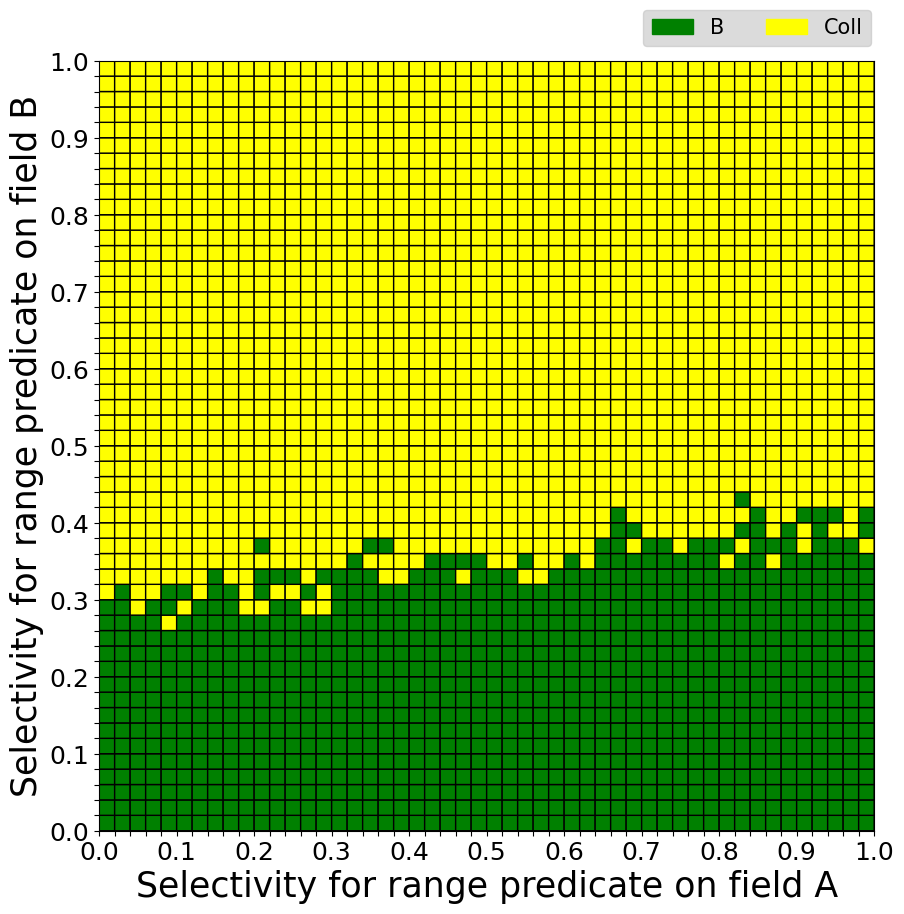
\includegraphics[width=0.30\textwidth]{images/results-without-covering-index/v\mdbver/comprehensive_practical_winner.png}}}
    \centering
    \subfigure[Chosen query plan with both attributes indexed: MongoDB never chooses a collection scan.]{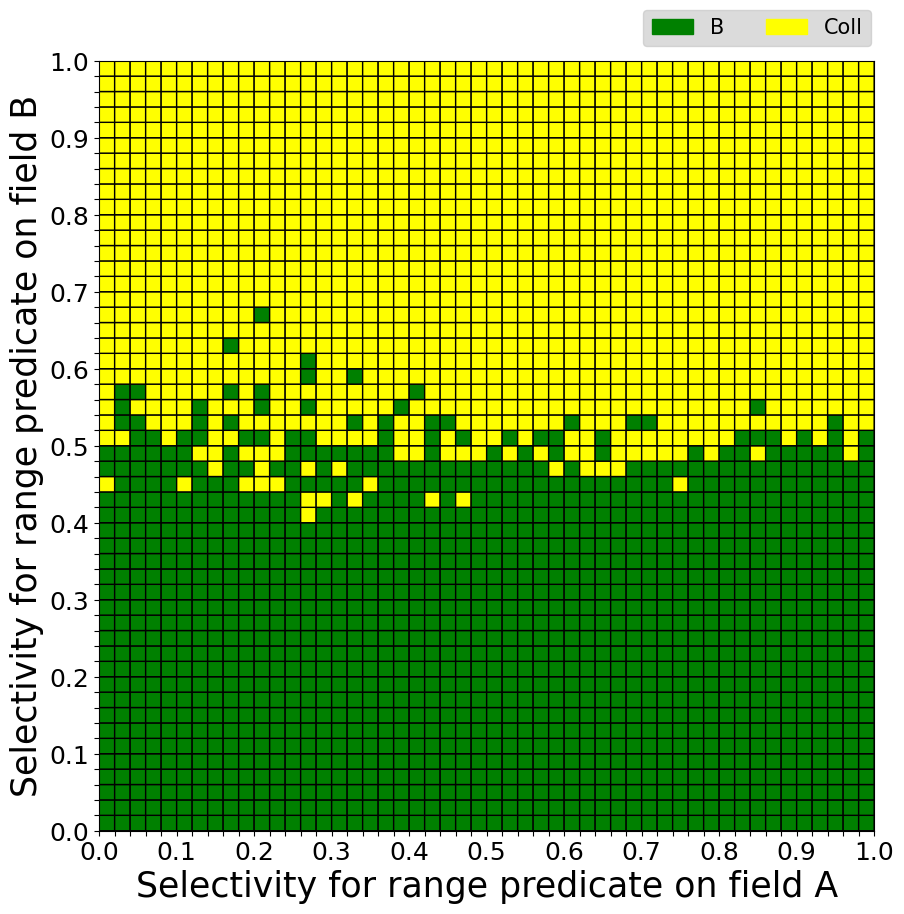
\includegraphics[height=\plotheight]{images/results-without-covering-index/v\mdbver/comprehensive_mongo_choice.png}\label{fig:mongo-bothindexed-choices}}
    \hfill
    \subfigure[Optimal query plan for different selectivities with both attributes indexed.]{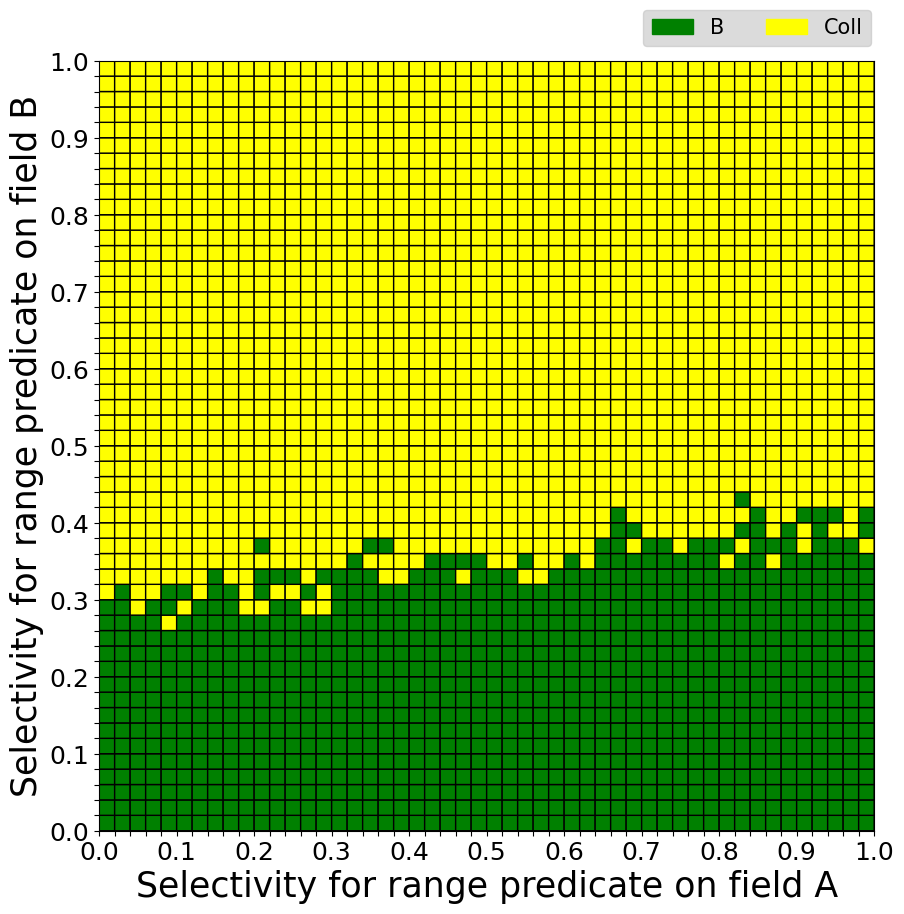
\includegraphics[height=\plotheight]{images/results-without-covering-index/v\mdbver/comprehensive_practical_winner.png}\label{fig:mongo-bothindexed-optimal}}
    \hfill
    \subfigure[Performance impact of MongoDB's sub-optimal choices.]{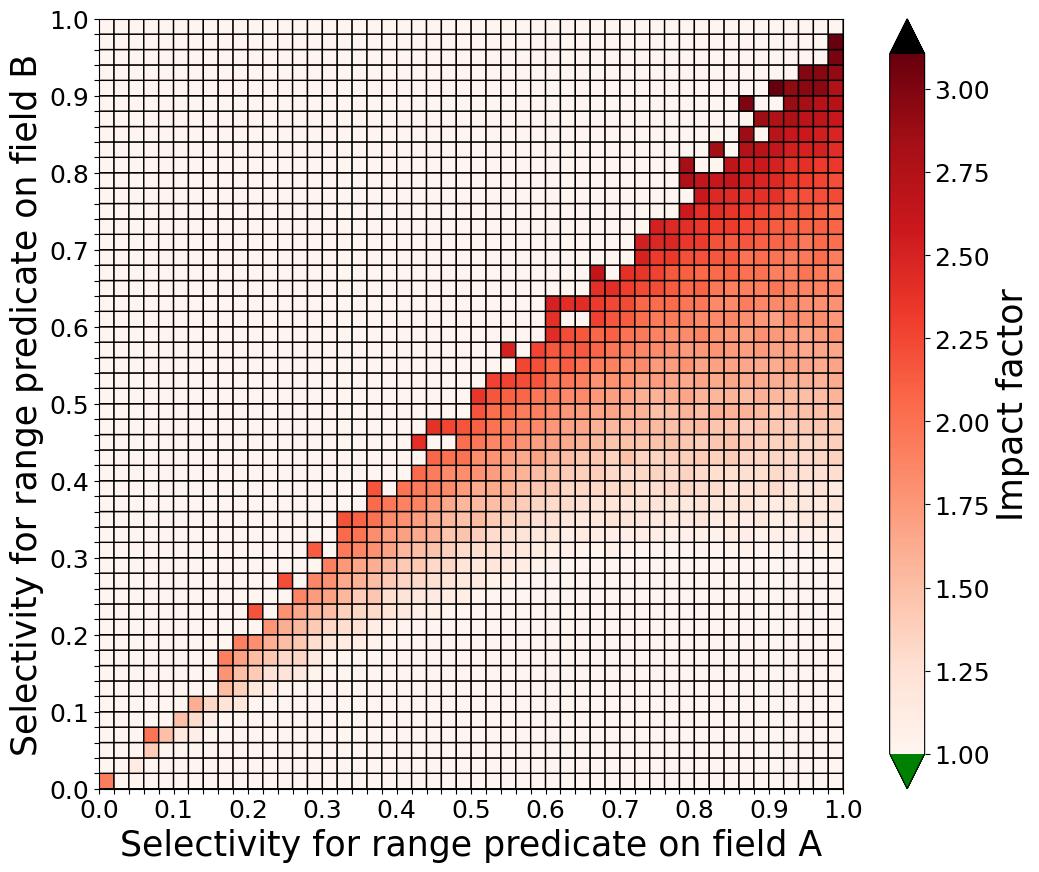
\includegraphics[height=\plotheight-1em]{images/results-without-covering-index/v\mdbver/comprehensive_summary_accuracy.png}\label{fig:mongo-bothindexed-perfimpact}}
    \vspace*{-0.75\baselineskip}
    \caption{Effectiveness of MongoDB's query optimizer with conjunctive filter queries and both attributes indexed.}
    \label{fig:bothindexed-evaluation}
\end{figure*}

\subsection{Visualization of Performance Impact}
We further want to assess how much query performance is impacted by the choices the optimizer makes. To do so, we determine for each query the ratio of the runtime of the plan chosen by the optimizer to the runtime of the plan that actually runs fastest for that query. We propose a heatmap presentation which we believe has not been used before for this aspect of optimizer effectiveness; we plot these ratios on the same discretized grid, with coordinates reflecting the selectivities, and we use a heatmap for the color, in which the color saturation corresponds to the ratio between runtime of the chosen plan and runtime of the truly optimal plan for that query.  If the query optimizer has chosen the optimal plan (a performance ratio of 1.0 between its choice and the optimal plan), we represent this with white pixels. 
But the darker the color of a box, the worse the performance impact of the query optimizer's (suboptimal) choice. An example of such a heat map visualizing the impact of \approachName performance is shown in Figure~\ref{fig:mongo-bothindexed-perfimpact}.

%The ideal baseline is directly related with the executiontime of the real best query plan among all candidate plans.That is to say, the execution time of a query should be the shortest with a real best query plan; it is impossibleto further improve the query performance through switchingother query execution strategies. The query execution time,our vital metric, can be obtained by inspecting queryexecution statistics. During the experiment, we extract the \verb|executionStats.executionTimeMillis| field to retrieve the wall-clock time in milliseconds required for the query plan evaluation and query execution.

%If there are multiple query plan candidates, we determine the real best candidate by measuring and comparing the execution time of each query plan candidate. As we mentioned in the section \ref{sec:hint}, MongoDB provides users a \verb|hint(<queryPlan>)| method to customize execution plan. We use this method to force the query optimizer to execute each candidate plan. After executing all query plans,the one with the shortest execution time is the real best query plan. We use the visualization technique explained in the section \ref{sec:vm} to visualize all real best plans in the 2D coordinate. Similar to the experiment in Part 2, we find the real best query plan through a majority vote. We repeat this experiment ten times to measure the mean execution time of the real best query plan. 

%In addition, we visualize the impact of the defect using a heatmap. The color of the pixel (i,j) in the heatmap is determine by the value of $\delta_{i,j}$. After recording the execution time of all real best query plans. We use the same technique to obtain the execution time of query plans selected by MongoDB V2. And then we can calculate the value of $\delta_{i,j}$ using the mean execution time of the query plans selected by MongoDB V2 and that of the real best query plans:

%\begin{equation}
%    \delta_{i,j} = \frac{\sum\limits_{n=1}^{N}t_{i,j,n}}{\sum\limits_{n=1}^{N}t_{i,j,n}^{'}}
%\end{equation}

%\begin{equation}
%    \delta_{i,j} = \frac{\sum\limits_{n=1}^{N}t_{i,j,n}}{\sum\limits_{n=1}^{N}t_{i,j,n}^{'}}
%\end{equation}

%\begin{equation}
%    \delta = \frac{t_{chosen}}{t_{optimal}}
%\end{equation}

%,where N is the number of repetition, $t_{i,j,n}^{'}$ is the execution time of the query plan at (i,j) selected by MongoDB V2 in the $nth$ repetition, and $t_{i,j,n}$ is the execution time of the real best query plan at (i,j) in the $nth$ repetition. 

%For each visualization, we express the overall performance difference ($\Delta_p$) between the ideal query plans and the actual ones in terms of mean query execution time. For the $(ith, jth)$ query, we denote the mean execution time of its optimal query plan as $\mu_{i,j}$ and that of the actual query plan as $\mu_{i,j}^{'}$.

%\begin{equation}
%    \Delta_p = \frac{\sum\limits_{j=0}^{D-1}(\sum\limits_{i=0}^{D-1}\mu_{i,j}^{'}) - \sum\limits_{j=0}^{D-1}(\sum\limits_{i=0}^{D-1}\mu_{i,j})}       {\sum\limits_{j=0}^{D-1}(\sum\limits_{i=0}^{D-1}\mu_{i,j})}
%\end{equation}

%\begin{equation}
%    \Delta_p = \frac{\sum\limits_{j=0}^{D-1}(\sum\limits_{i=0}^{D-1}t_{i,j}^{'}) - \sum\limits_{j=0}^{D-1}(\sum\limits_{i=0}^{D-1}t_{i,j})}       {\sum\limits_{j=0}^{D-1}(\sum\limits_{i=0}^{D-1}t_{i,j})}
%\end{equation}

%$D$ is the dimension of the grid. A negative value of ($\Delta_p$) indicates the performance is worse than the optimal case.

%The accuracy of the query optimizer can be calculated as:
%\begin{equation}
%    accuracy = \frac{\text{correctly predicted cases}}{\text{total number of cases}} \times 100\%
%\end{equation}

%ADF got to here with edits